\documentclass[10pt,letterpaper]{article}
\renewcommand{\rmdefault}{ptm}

\usepackage[left=1in,right=1in,top=1in,bottom=1in]{geometry} 
\usepackage{amsmath}
\usepackage{amsfonts}
\usepackage{amsthm}
\usepackage{amssymb}
\usepackage{polynomial}
\usepackage{layouts}

\usepackage{enumerate}

\usepackage{syntax}
\usepackage{gensymb}
\usepackage{cancel}
\usepackage{calc}
\usepackage{enumerate}
\usepackage{xcolor}

\usepackage{minted}

\usepackage[version=0.96]{pgf}
\usepackage{tikz}
\usetikzlibrary{arrows,shapes,automata,backgrounds,petri,positioning}
\usetikzlibrary{decorations.pathmorphing}
\usetikzlibrary{decorations.shapes}
\usetikzlibrary{decorations.text}
\usetikzlibrary{decorations.fractals}
\usetikzlibrary{decorations.footprints}
\usetikzlibrary{shadows}
\usetikzlibrary{calc}
\usetikzlibrary{spy}
\usetikzlibrary{matrix}

\usepackage{tikz-qtree}

\setcounter{tocdepth}{2}
\setcounter{secnumdepth}{4}
\usepackage[bookmarksopen,bookmarksdepth=3]{hyperref}
\usepackage{titlesec}


%define new colors
\definecolor{dark-red}{rgb}{0.8,0.15,0.15}
\definecolor{dark-blue}{rgb}{0.15,0.15,0.7}
\definecolor{medium-blue}{rgb}{0,0,0.5}
\definecolor{dark-green}{rgb}{0.2,0.7,0.7}

%set up color for table of contents
\hypersetup{
    colorlinks, linkcolor={dark-green},
    citecolor={dark-blue}, urlcolor={medium-blue}
}

\usepackage{tocloft}

%preven linebreak between subsection header and its content
\titleformat{\subsection}[runin]{\normalfont\bfseries}{\thesubsection.}{2pt}{}
%\titleformat{\section}[runin]{\normalfont\bfseries\filcenter}{\thesection.}{5pt}{}


\titleformat{\section}[block]
{\normalfont\sffamily\LARGE}
{\thesection}{.2em}{\titlerule\\[.2ex]\bfseries}

%title
\title{\textbf{Math 350 - Advanced Calculus \\ Homework 8}}
\author{Chan Nguyen}

%set numwidth of section
\setlength{\cftsecnumwidth}{1.5cm} 
%make subsection numwidth different than as section
\setlength{\cftsubsecnumwidth}{3cm}
%make subsection indent the same as section
\setlength{\cftsubsecindent}{\cftsecindent} 

\newcommand{\sol}{\textbf{Solution}}

\usepackage{tikz}
\usetikzlibrary{matrix}
\usetikzlibrary{shapes,backgrounds}

\makeatletter
\newcommand{\DESCRIPTION@original@item}{}
\let\DESCRIPTION@original@item\item
\newcommand*{\DESCRIPTION@envir}{DESCRIPTION}
\newlength{\DESCRIPTION@totalleftmargin}
\newlength{\DESCRIPTION@linewidth}
\newcommand{\DESCRIPTION@makelabel}[1]{\llap{#1}}%
\newcommand{\DESCRIPTION@item}[1][]{%
  \setlength{\@totalleftmargin}%
       {\DESCRIPTION@totalleftmargin+\widthof{\textbf{#1 }}-\leftmargin}%
  \setlength{\linewidth}
       {\DESCRIPTION@linewidth-\widthof{\textbf{#1 }}+\leftmargin}%
  \par\parshape \@ne \@totalleftmargin \linewidth
  \DESCRIPTION@original@item[\textbf{#1}]%
}
\newenvironment{DESCRIPTION}
  {\list{}{\setlength{\labelwidth}{0cm}%
           \let\makelabel\DESCRIPTION@makelabel}%
   \setlength{\DESCRIPTION@totalleftmargin}{\@totalleftmargin}%
   \setlength{\DESCRIPTION@linewidth}{\linewidth}%
   \renewcommand{\item}{\ifx\@currenvir\DESCRIPTION@envir
                           \expandafter\DESCRIPTION@item
                        \else
                           \expandafter\DESCRIPTION@original@item
                        \fi}}
  {\endlist}
\makeatother

\begin{document}

\tableofcontents 
\maketitle

\setlength{\parindent}{0pt}
\setlength{\parskip}{1ex}
	\phantomsection
	\subsection*{{\color{purple}\underline{Problem 1}}}
	\addcontentsline{toc}{subsection}{\numberline{}Problem 1}
	Let $\complement[0, 1]$ denote set of continuous functions on interval $[0, 1]$. If
	$f \in \complement[0, 1]$, define
	$$||f|| = \sup\{|f(x)| : 0 \leq x \leq 1\}$$
	\begin{enumerate}[(i)]
		\item Prove that $||\lambda f|| = |\lambda|||f||$, for every real number $\lambda$ and every 
		$f \in \complement[0, 1]$.
		\begin{proof}
		We claim that $|\lambda \cdot f(x)| = |\lambda| \cdot |f(x)|$ for all $x \in \mathbb{R}$ and 
		for all $\lambda \in \mathbb{R}$. There are two cases to consider,
		\begin{itemize}
			\item If $\lambda$ and $f(x)$ have the same sign, then 
			$|\lambda \cdot f(x)| = \lambda \cdot f(x) = |\lambda| \cdot |f(x)|$
			\item If $\lambda$ and $f(x)$ have opposite sign, then
			$|\lambda \cdot f(x)| = -(\lambda \cdot f(x))$ where
			$|\lambda| \cdot |f(x)| = -(\lambda \cdot f(x))$ 
		\end{itemize}
		Thus in both cases, $|\lambda \cdot f(x)| = |\lambda| \cdot |f(x)|$.
		Now go back to our problem, we have that 
		$$||f|| = \sup\{|f(x)| : 0 \leq x \leq 1\}$$
		Hence $$||\lambda \cdot f|| = \sup\{|\lambda \cdot f(x)| : 0 \leq x \leq 1 \} = |\lambda| \cdot 
		\sup\{|f(x)| : 0 \leq x \leq 1\} = |\lambda| ||f||$$
		\end{proof}
		
		\item Prove that $||f|| = 0$ if and only if $f(x) = 0$ for all $x \in [0, 1]$.
		\begin{proof}
		We have $||f|| = 0 \Rightarrow \sup\{|f(x)| : 0 \leq x \leq 1\} = 0$. By definition 
		of $\sup$ we have $|f(x)| \leq 0$ for all $x$, and by definition of absolute value, we have
		$0 \leq f(x)$. Combine these two inequalities, $0 \leq |f(x)| \leq 0$ implies $f(x) = 0$
		for all $x \in [0, 1]$.		
		\end{proof}
				
		\item Prove that $||f + g|| \leq ||f|| + ||g||$ for every $f, g \in \complement[0, 1]$.
		\begin{proof}
			We have $||f + g|| = \sup\{|(f + g)(x)| : 0 \leq x \leq 1 \}$. By definition of $\sup$, 
			for all $\epsilon > 0$, there exists some $a \in [0, 1]$ such that
			$$||f + g|| - |f + g|(a) < \epsilon$$
			which implies that
			$$||f + g|| - (|f|(a) + |g|(a)) < \epsilon$$
			Since $|f|(a) \leq ||f||$ and $|g|(a) \leq ||g||$, it follows that
			$$||f + g|| - (||f|| + ||g||) < \epsilon$$
			Since this is true for every $\epsilon > 0$, it follows that
			$||f + g|| \leq ||f|| + ||g||$.
		\end{proof}				
		
		\item Find $f, g \in \complement[0, 1]$ such that $||f + g|| \neq ||f|| + ||g||$.
		This follows from (iii).
	\end{enumerate}
	
	\phantomsection
	\subsection*{{\color{purple}\underline{Problem 2}}}
	\addcontentsline{toc}{subsection}{\numberline{}Problem 2}
	Prove that if $A$ and $B$ are connected subsets of $\mathbb{R}$ and $A \cap B = \emptyset$, then
	$A \cup B$ is connected.
	\begin{proof}
		Let $S = A \cup B$ is disconnected since $A \cap B = \emptyset$, $A \neq \emptyset$ and $B \neq \emptyset$,
		where $A, B$ are open. Suppose that $A$ and $B$ are open and connected, $A \cap B = \emptyset$ and 
		$S = A \cup B$ is disconnected. Then $S \subset (U \cup V)$, where $U, V$ are open in $\mathbb{R}$, 
		$U \cap S \neq \emptyset$, $V \cap S \neq \emptyset$, and $U \cap V \cap S = \emptyset$. Since $A$ is connected,
		and $A \subset U \cup V$, we must have $U \cap A = \emptyset$, or $V \cap B = \emptyset$. That is, either
		$A \subset U$ or $A \subset V$. Similarly, we must have either $B \subset U$, or $B \subset V$. In any case,
		we always have $(A \cap B) \subset (U \cap V)$. Since $A \cap B = \emptyset$, this contradicts the fact that
		$S \cap U \cap V = \emptyset$. Thus $S$ is connected.
	\end{proof}
	
	\phantomsection
	\subsection*{{\color{purple}\underline{Problem 3}}}
	\addcontentsline{toc}{subsection}{\numberline{}Problem 3}
	True of False: If $f$ is continuous and $S$ is connected, then $f^{-1}S$ is connected.
	
	\phantomsection
	\subsection*{{\color{purple}\underline{Problem 4}}}
	\addcontentsline{toc}{subsection}{\numberline{}Problem 4}
	Prove that if $f$ is continuous on an interval $J$ and $f(x)$ is rational for every $x$ in $J$,
	then $f$ is constant on $J$.
	\begin{proof}
		Suppose that $f$ is not constant, so for $a, b \in J$, $f(a) \neq f(b)$. Then by Intermediate Value
		Theorem, for any $c \in (f(a), f(b)$ there exists $x \in (a, b)$ such that $f(x) = c$. This contradicts
		that $f$ takes on all rational numbers only because between 2 rational numbers $f(a), f(b)$, there are
		irrational numbers. 	
	\end{proof}
	
	
	\phantomsection
	\subsection*{{\color{purple}\underline{Problem 5}}}
	\addcontentsline{toc}{subsection}{\numberline{}Problem 5}
	Suppose $f$ is continuous on $[a, b]$ and $f(a) < 0 < f(b)$.
	\begin{enumerate}[(i)]
	\item Prove that either $f(\dfrac{a+b}{2}) = 0$ or $f$ has different signs at the end points
	$[a, (a+b)/2]$ or $f$ has different signs at the end points of $[(a+b)/2, b]$. 
	If $f(\dfrac{a+b}{2}) \neq 0$, let $I_1$ be one of the two intervals on which $f$ 
	has different signs at the endpoints. Now bisect $I_1$. Then either $f$ is $0$ at the midpoint,
	or $f$ has opposite signs at the endpoints of one of the two intervals into which $I_1$ is
	bisected. Let $I_2$ be such an interval. Continue this way to define $I_n$ for each natural
	number $n$ (unless $f$ is 0 at some midpoint).
	\begin{proof}
	If $f((a+b)/2) \neq 0$, then this number is either $> 0$ and $f$ has different signs at the endpoints
	of $[a, (a+b)/2]$, or $< 0$ and $f$ has different signs at the endpoints of $[(a + b)/2,b]$.
	\end{proof}
	
	\item Prove that there is a point $x \in (a, b)$ where $f(x) = 0$.
	\begin{proof}
	Let $c$ be in each interval $I_n$. If $f(c) < 0$, then there is some $\delta > 0$
	such that $f(x) < 0$ for all $x \in [a, b]$ with $|x - c| < \delta$. Choose $n$
	with $\dfrac{1}{2^n} < \delta$. Since $c$ is in $I_n$ which has total length of
	$\dfrac{1}{2^n}$, it follows that all points $x$ of $I_n$ satisfy $|x - c| < \delta$.
	This contradicts the fact that $f$ changes sign on $I_n$. Similarly, we cannot have
	$f(c) > 0$, so $f(c) = 0$.
	\end{proof}
	
	\item Use the scheme described in (i) and (ii) to approximate the solution of
	$x^3 + 6x - 2 = 0$ with an error smaller than $\dfrac{1}{100}$.
	\begin{proof}
		If $f(x) = x^3 + 6x - 2$, then $f(0) = -2$ and $f(1/3) > 0$. Let $[a, b] = [0, 1/3]$. Since 
		length $I_n = \dfrac{1}{3} \cdot 2^n$ and $3 \cdot 2^5 < 100 < 3 \cdot 2^6$, any of the endpoints
		of $I_6$ will approximate the solution of $f(x) = 0$ with an error smaller than
		$1/100$.
	\end{proof}
	
	
	\end{enumerate}
	
	
	\phantomsection
	\subsection*{{\color{purple}\underline{Problem 6}}}
	\addcontentsline{toc}{subsection}{\numberline{}Problem 6}
	Find an integer $n$ such that the polynomial equations $x^3 - x + 3 = 0$ has a solution
	between $n$ and $n + 1$.
	\begin{proof}
	By Polynomial Root Theorem, we know that $f(x) = x^3 - x + 3$ has a solution because $n = 3$ is odd.
		Apply Location of Root Theorem, we want to find $n$ and $n + 1$ such that $\mathrm{sign}(f(n)) \neq \mathrm{sign}(f(n+1))$,
		then the solution must be between $[n, n+1]$. Since the first term $x^3$ is much larger than other term, to make $f(x)$ negative,
		we obviously need a negative $x$, we could try \\
		$f(-2) = (-2)^3 - (-2) + 3 = -8 + 4 + 3 = -1$ \\
		$f(-1) = (-1)^3 - (-1) + 3 = -1 + 1 + 3 = 3$ \\
		It follows that $f(-2) < 0 < f(-1)$, thus the solution is between $[-2, -1]$.
	\end{proof}
	
	\phantomsection
	\subsection*{{\color{purple}\underline{Problem 7}}}
	\addcontentsline{toc}{subsection}{\numberline{}Problem 7}
	Prove that there is some number $x$ such that $\sin(x) = x - 1$.
	\begin{proof}
		Let $f(x) = x − 1 − \sin(x)$. Then $f(0) = −1 < 0$ and $f(\pi/2) = \pi/2 > 0$, so there is $
		x \in (0, \pi/2)$ such that
		$f(x) = 0 \Leftrightarrow \sin(x) = x − 1$.
	\end{proof}
	
	\phantomsection
	\subsection*{{\color{purple}\underline{Problem 8}}}
	\addcontentsline{toc}{subsection}{\numberline{}Problem 8}
	\text{ }
	\begin{enumerate}[(a)]
		\item Suppose that $f$ is continuous on the interval $[0, 1]$ and that $0 \leq f(x) \leq 1$ for 
		all $x \in [0, 1]$. Prove that $f(x) = x$ for some numbers $x \in [0, 1]$.
		\begin{proof}
		Recall, \\
		\textbf{Location of Roots Theorem. } If $f$ is continuous on $[a,b]$ and $f(a) < 0 < f(b)$, then
		there is some $x \in [a, b]$ such that $f(x) = 0$. \\
		Our goal is to apply this Theorem for $f(x) - x$. Let $g(x) = f(x) - x$, we have 
		that $f(1) - 1 \leq 0$ and $f(0) - 0 \geq 0$. \\ 
		If the "$=$" occurs,
		then $f(1) - 1 = 0 \Rightarrow f(1) = 1$ and $f(0) - 0 = 0 \Rightarrow f(0) = 0$ which is
		what we want to show. Otherwise, we have $h(1) < 0$ and $h(0) > 0$ which implies
		there is some $x \in [0, 1]$ such that $h(x) = 0$ by Location of Roots Theorem. Hence,
		$f(x) - x = 0 \Leftrightarrow f(x) = x$ for some $x \in [0, 1]$. 
		\end{proof}
		
		\item Let $f$ be continuous and bounded above and below on $\mathbb{R}$. Prove that there is
		some number $x$ such that $f(x) = x$.
		\begin{proof}
			Let $m, n$ be lower bound and upper bound of $f$ respectively, then $f(x) \geq m, f(x) \leq n$
			for all $x \in \mathbb{R}$. If $f(x) = m$ or $f(x) = n$ for all $x$, then $f(x)$ is constant,
			so $f(x) = x$ is trivially true. If not, there is some $x$ such that
			$m < f(x) < n$. Using the same idea from part (a), we consider
			$$g(x) = f(x) - x$$
			We have that $g(m) = f(m) - m > 0$ and $g(n) = f(n) - n < 0$ so apply Location of Roots Theorem,
			we have there is some $x \in \mathbb{R}$ such that $g(x) = 0 \Leftrightarrow f(x) = x$ which 
			was what we want to show. 
			
			
		\end{proof}				
	\end{enumerate}
	
	
	\phantomsection
	\subsection*{{\color{purple}\underline{Problem 9}}}
	\addcontentsline{toc}{subsection}{\numberline{}Problem 9}
	One morning, exactly at sunrise, a Buddhist monk began to climb a tall mountain. The narrow
path, no more than a foot or two wide, spiraled around the mountain to a glittering temple at the summit
The monk ascended the path at varying rates of speed stopping along the way to rest and to eat the
dried fruit he carried with him. He reached the temple shortly before sunset. After several days of fasting
and meditation he began his journey back along the same path, starting at sunrise and again walking at
variable speeds with many pauses along the way. His average speed descending was, of course, greater than
his average climbing speed.
Prove that there is a spot along the path that the monk will occupy on both trips at precisely the same
time of day. (Martin Gardner, in \emph{My Best Mathematical Puzzles} Dover 1994.)
	
	\phantomsection
	\subsection*{{\color{purple}\underline{Problem 10}}}
	\addcontentsline{toc}{subsection}{\numberline{}Problem 10}
	A function $f$ defined on an interval $I$ has the Intermediate Value Property on $I$ if
	for any two numbers $a < b$ in $I$ and every $y$ strictly between $f(a)$ and $f(b)$, there is
	$c \in (a, b)$ such that $f(c) = y$.
	\begin{enumerate}[(i)]
		\item Prove that the function $f$ given by $f(x) = \sin(1/x)$ if $x \neq 0$ and $f(0) = 0$ has the
		Intermediate Value Property on the interval $[0, B]$ for any $B > 0$.
\begin{proof}
	If $0 < a < b$ are two numbers in $[0, B]$, then we apply the Intermediate Value Theorem to $f(x) = \sin(1/x)$
	on $[a, b]$ because $f$ is continuous on $[a, b]$. However, if $0 = a < b$ and $x$ is strictly between 
	$0 = f(0)$ and $f(b)$, let $n$ be a natural number such that $\dfrac{2}{b} < (2n+1) \cdot \pi$ so
	that the interval
	$$I = \bigg[\dfrac{2}{2n + 3} \cdot \pi, \dfrac{2}{2n + 1} \cdot \pi\bigg]$$ is contained in $[0, b]$. 
	The function $f(x) = \sin(1/x)$ is continuous on I and takes on the values $1$ and $−1$ at the endpoints of $I$. 
	Since $−1 \leq f(x) \leq 1$, the Intermediate Value Theorem
applied to $f$ on $I$ implies that given any $y$ such that $−1 < y < 1$, there is $c$ in $I$ such that 
$f(c) = y$. In particular, if $y$ is strictly between $f(a)$ and $f(b)$, then $−1 < y < 1$ also, 
and $c$ in $I$ satisfies $0 = a < c < b$, as desired.	
\end{proof}						
		\item Prove that if $f$ is non-decreasing on the interval $I$ and has the Intermediate Value 
		Property on $I$, then $f$ is continuous on $I$. (Adopting the terminology of the textbooks, 
		$f$ is said to be increasing on $I$ if $f(x) < f(y)$ whenever $x < y$ in $I$; it is said
		to be non-decreasing if $f(x) \leq f(y)$ whenever $x < y$.
\begin{proof}
Suppose that there is $a$ in $I$ where $f$ fails to be continuous. Then there is a sequence $(x_n)$ in $I$ 
such that $x_n \rightarrow a$ but $f(x_n)$ does not converge to $f(a)$. We may assume, 
by taking a subsequence if necessary, that $x_n$
increases (or decreases) to $a$. 
	Then $f(x_n)$ is non decreasing and bounded above by $f(a)$, thus it converges to $a$
	number $p$ with $p < f(a)$. 
	Let $q$ be a number such that $p < q < f(a)$. For each $x_n$ we have $f(x_n) \leq p < q$, 
	so the Intermediate Value Property of $f$ on the interval $[x_n, a]$ implies the existence 
	of $y_n$ in $(x_n, a)$ such that $f(y_n) = q$. The sequence $(y_n)$ 
	converges to a and $f(y_n) = q$ for all $n$. 
	Since $x_n$ also converges to $a$, given $n$ there is $m$ such
	that $y_n < x_m$, but $f(y_n) = q > p \geq f(x_m)$, contradicting that $f$ is non decreasing.

\end{proof}		
		
		
	\end{enumerate}
	
	\phantomsection
	\subsection*{{\color{purple}\underline{Problem 11}}}
	\addcontentsline{toc}{subsection}{\numberline{}Problem 11}
	Let $f(x) = x^2$ if $x$ is rational, and $f(x) = 0$ if $x$ is not rational. Prove that $f$
	is differentiable at $0$.
	$$f(x) = 
	\begin{cases}
		x^2 &, \text{ if } x \text{ is rational } \\
		0   &, \text{ if } x \text{ is not rational }
	\end{cases}
	$$
	\begin{proof}
	To prove that $f$ is differentiable at $0$, we want to show that:
	$$\displaystyle\lim_{h\to 0} \dfrac{f(0 + h) - f(0)}{h} 
	= \displaystyle\lim_{h\to 0} \dfrac{f(h) - f(0)}{h}
	\text{ exists } $$
	Since $0$ is both rational and irrational we have that $f(0) = 0$, it reduces to prove
	 $\displaystyle\lim_{h\to 0} \dfrac{f(h)}{h}$ exists.
	On the other hand, we have
	$$\dfrac{f(x)}{x} = 
	\begin{cases}
		\dfrac{x^2}{x} = x &, \text{ if } x \text{ is rational } \\
		0 &, \text{ if } x \text{ is not rational }
	\end{cases}
	$$
	So in either case, as $x \rightarrow 0$, $\dfrac{f(x)}{x} = 0$, in other words
	$\displaystyle\lim_{h\to 0} \dfrac{f(h)}{h} = 0$, so $f'(0)$ exists or $f$ is
	differentiable at $0$.
	
	\end{proof}
	
	\phantomsection
	\subsection*{{\color{purple}\underline{Problem 12}}}
	\addcontentsline{toc}{subsection}{\numberline{}Problem 12}	
	Let $f$ be a function such that $|f(x)| \leq x^2$ for all $x$. Prove that $f$ is differentiable
	at $0$ and find $f'(0)$.
	\begin{proof}
		Since $|f(x)| \leq x^2$ for all $x$, we have $0 \leq |f(x)| \leq 0^2 = 0$ which implies 
		$f(0) = 0$. 
		Also since $\bigg|\dfrac{f(h)}{h}\bigg| \leq \dfrac{h^2}{|h|}$, it follows
		that $ -h \leq \dfrac{f(h) - f(0}{h} \leq -h \Rightarrow \displaystyle\lim_{h\to 0}\dfrac{f(h)}{h} = 0$, i.e, $f'(0) = 0$.
	\end{proof}
	
	
	\phantomsection
	\subsection*{{\color{purple}\underline{Problem 13}}}
	\addcontentsline{toc}{subsection}{\numberline{}Problem 13}
	Find $f'(x)$ for $-1 < x < 1$ if $f(x) = \sqrt{1 - x^2}$.
	\begin{proof}
		Apply Chain rule, we have
		$$f'(x) = \dfrac{1}{2}(1 - x^2)^{1/2 - 1} \cdot (-2x) = \dfrac{-x}{\sqrt{1 - x^2}}$$
	\end{proof}
	
	\phantomsection
	\subsection*{{\color{purple}\underline{Problem 14}}}
	\addcontentsline{toc}{subsection}{\numberline{}Problem 14}
	If $f$ is differentiable three times and $f'(x) \neq 0$, the Schwartz derivative of $f$ at $x$
	is defined to be 
	$$Sf(x) = \dfrac{f'''(x)}{f'(x)} - \dfrac{3}{2} \bigg(\frac{f''(x)}{f'(x)}\bigg)^2$$
	\begin{enumerate}[(i)]
		\item Show that 
		$$S(f \circ g) = [S f \circ g] \cdot (g')^2 + Sg$$
		Consider
		$$(f \circ g)'(x) = f'(g(x)) \cdot g'(x)$$
		$$(f \circ g)''(x) = f''(g(x)) \cdot g'(x)^2 + f'(g(x)) \cdot g''(x)$$
		\begin{eqnarray*}
		(f \circ g)'''(x) 
		&=&
		[f'''(g(x)) \cdot g'(x)^3 + 2f''(g(x)) \cdot g'(x)g''(x)] 
		+ [f''(g(x)) \cdot g'(x)g''(x) + f'(g(x)) \cdot g'''(x)] \\
		&=& f'''(g(x)) \cdot g'(x)^3 + 3f''(g(x)) \cdot g'(x)g''(x) + f'(g(x)) g'''(x)
		\end{eqnarray*}
		Plug it back into the the Schwartz derivative, we have
	\begin{eqnarray*}
		Sf(x) &=& \dfrac{f'''(x)}{f'(x)} - \dfrac{3}{2} \bigg(\frac{f''(x)}{f'(x)}\bigg)^2 \\
&=& \dfrac{(f \circ g)'''}{(f \circ g)'} - \dfrac{3}{2} \bigg(\dfrac{(f \circ g)''}{(f \circ g)'}\bigg)^2 \\
&=& \dfrac{(f''' \circ g)g'^2}{f' \circ g} + \dfrac{3(f'' \circ g)g''}{f' \circ g} + \dfrac{g'''}{g'}
- \dfrac{3}{2} \bigg( \dfrac{(f'' \circ g) \cdot g'}{f' \circ g} + \dfrac{g''}{g'}\bigg)^2\\
&=& \dfrac{(f''' \circ g)g'^2}{f' \circ g} + \dfrac{3(f'' \circ g)g''}{f' \circ g} + \dfrac{g'''}{g'}
- \dfrac{3}{2} \bigg( \dfrac{(f'' \circ g) \cdot g'}{f' \circ g} \bigg)^2 
- 3 \dfrac{(f'' \circ g)g''}{f' \circ g} - \dfrac{3}{2} \bigg( \dfrac{g''}{g'} \bigg)^2 \\
&=& \bigg[\dfrac{f'''}{f'} \circ g - \dfrac{3}{2} \dfrac{f'' \circ g}{f' \circ g}\bigg] \cdot g'^2
+ \dfrac{g'''}{g'} - \dfrac{3}{2} \bigg(\dfrac{g''}{g'}\bigg)^2 \\
&=& [Sf \circ g] \cdot g'^2 + Sg\\	
	\end{eqnarray*}
			
		\item Show that if $f(x) = \dfrac{ax + b}{cx + d}$ with $ad - bc \neq 0$, then 
		$Sf = 0$, and consequently $S(f \circ g) = Sg$.
\begin{proof}
	Consider
	$$f'(x) = \dfrac{a(cx + d) - c(ax + b)}{(cx + d)^2} = \dfrac{ad - bc}{(cx + d)^2}$$
	$$f''(x) = \dfrac{-2c(ad - bc)}{(cx + d)^3}$$
	$$f'''(x) = \dfrac{6c^2(ad - bc)}{(cx + d)^4}$$
	Hence,
	$$Sf = \dfrac{6c^2}{(cx + d)^2} - \dfrac{3}{2}\bigg(\dfrac{-2c}{cx + d}\bigg)^2 = 0$$
\end{proof}
	\end{enumerate}
	
	\phantomsection
	\subsection*{{\color{purple}\underline{Problem 15}}}
	\addcontentsline{toc}{subsection}{\numberline{}Problem 15}
	A function $f$ is Lipschitz of order $\alpha$ at $x$ is, there is a constant $C$ such that
	\[
		|f(x) - f(y)| \leq C|x - y|^{\alpha}
	\]		
	for all $y$ in an interval around $x$. Then function $f$ is Lipschitz of order $\alpha$
	on an interval if $(1)$ holds for all $x$ and $y$ in the interval.
	\begin{enumerate}[(a)]
		\item If $f$ is Lipschitz of order $\alpha > 0$ at $x$, then $f$ is continuous at $x$.
\begin{proof}
	Since $|f(x) - f(x + h)| \leq C|h|^{\alpha}$ it follows that $\displaystyle\lim_{h\to 0}
	f(x+h) = f(x)$.
\end{proof}
		\item If $f$ is Lipschitz of order $\alpha > 0$ on an interval, then $f$ is uniformly
		continuous on this interval.
\begin{proof}
Given $\epsilon > 0$ choose $\delta = \bigg(\dfrac{\epsilon}{C}\bigg)^{1/\alpha}$ so that
$\delta^{\alpha} = \dfrac{\epsilon}{C}$. Then for all $x$ and $y$ in the interval 
with $|x - y| < \delta$ we have
	$$|f(x) - f(y)| \leq C|x - y|^{\alpha} < C \cdot \dfrac{\epsilon}{C} = \epsilon$$
\end{proof}
	\item If $f$ is differentiable at $x$, then $f$ is Lipschitz of order $1$ at $x$.
	\begin{proof}
	If $f$ is differentiable at $x$, then 
	$$\displaystyle\lim_{y\to x} \dfrac{f(y) - f(x)}{y - x} = f'(x)$$
	so for all $y$ in some interval around $x$ we have that
	$$\bigg| \dfrac{f(y) - f(x)}{y - x} - f'(x) \bigg| < 1$$ 	
	Hence,
	$$\bigg| \dfrac{f(y) - f(x)}{y - x} \bigg| < 1 + |f'(x)|$$	
	or 
	$$|f(y) - f(x)| \leq (1 + |f'(x)|)|y - x|$$
	so we can choose $C = 1 + |f'(x)|$ or we $C = \epsilon + |f'(x)|$ for 
	any $\epsilon > 0$. The converse is not true though, for example $f(x) = x$.	
	\end{proof}		
	
	
	\item If $f$ is Lipschitz of order $\alpha > 1$, then $f$ is differentiable at $x$ and
		$f'(x) = 0$.
	\begin{proof}
	 We have that 
	 $$f'(x) = \displaystyle\lim_{y\to x}\dfrac{f(y) - f(x)}{y - x}$$
	 Now consider 
	 $$\bigg|\dfrac{f(y) - f(x)}{y - x}\bigg| \leq |x - y|^{n-1}$$
	 and $\lim_{y\to x} |x - y|^{n-1} = 0$ since $n - 1 > 0$. Consequently
	 $f'(x) = 0$ for all $x$ and so $f$ is constant.
	 	
	\end{proof}
	
	\end{enumerate}
		
	\phantomsection
	\subsection*{{\color{purple}\underline{Problem 16}}}
	\addcontentsline{toc}{subsection}{\numberline{}Problem 16}
	Let $a > 0$. Show that the maximum value of 
	$$f(x) = \dfrac{1}{1 + |x|} + \dfrac{1}{1 + |x - a|}$$
	is $\dfrac{2 + a}{1 + a}$. Consider the interval $(-\infty, 0), (0, a)$ and $(a, \infty)$
	separately.
	\begin{proof}
$$f(x) =
\begin{cases}
	\dfrac{1}{1 - x} + \dfrac{1}{1 + a - x} &, x < 0 \\
	\dfrac{1}{1 + x} + \dfrac{1}{1 + a - x} &, 0 < x < a \\
	\dfrac{1}{1 + x} + \dfrac{1}{1 + x - a} &, a < x
\end{cases}
$$	
So the derivative is
$$f'(x) =
\begin{cases}
	\dfrac{1}{(1-x)^2}    + \dfrac{1}{(1 + a - x)^2} &, x < 0 \\
	\dfrac{-1}{(1 + x)^2} + \dfrac{1}{(1 + a - x)^2} &, 0 < x < a \\
	\dfrac{-1}{(1 + x)^2} - \dfrac{1}{(1 + x - a)^2} &, a < x
\end{cases}
$$
	Thus $f$ is increasing on $(-\infty, 0]$ and decreasing on $[a, \infty)$ so the maximum 
	of $f$ on $[0, a]$ is the maximum on $\mathbb{R}$. If $f'(x) = 0$ for $x \in (0, a)$ then
	$$(1 + x)^2 - (1 + a - x)^2 = 0$$
	whose only solution is $x = \dfrac{a}{2}$. Since
	$$f(\dfrac{a}{2}) = \dfrac{4}{2 + a} < \dfrac{2 + a}{1 + a} = f(0) = f(a)$$
	The maximum value is $\dfrac{2 + a}{1 + a}$.
	\end{proof}
	
	\phantomsection
	\subsection*{{\color{purple}\underline{Problem 17}}}
	\addcontentsline{toc}{subsection}{\numberline{}Problem 17}
	Find the length of the longest ladder that can be moved around a right-angle 
	corner from a corridor of width $a$ to a corridor of width $b$.
	\begin{proof} 
	\text{ } \\
	
	\begin{tikzpicture}
	\draw (1, 1) -- (8, 1);
	\draw (3, 0) -- (8, 0);
	\draw (3, 0) -- (3, -4);
	\draw (1, 1) -- (1, -4);
	
	\draw[red,<<->>] (1, -2) -- (4, 1);
	\draw[dashed] (1, -2) -- (3, -2);
	\draw[blue,<->] (3, -0.2) -- (4, -0.2) node[xshift=-4mm,yshift=-2mm] {$x$};
	
	\draw[blue,<->] (3.2, 0) -- (3.2, -2) node[xshift=2mm,yshift=5mm] {$y$};
	\draw[dashed] (4, 1) -- (4, 0);
	
	\draw[red,<<->>] (3, -3) -- (1, -3) node[xshift=1cm,yshift=3mm] {$a$};
	
	
	\draw[red,<<->>] (6, 0) -- (6, 1) node[xshift=2mm,yshift=-5mm] {$b$};
	\end{tikzpicture}
	\text{ } \\
	We note that the ratio $\dfrac{b}{x} = \dfrac{y}{a}$, so the length of ladder
	is 
$$L = \sqrt{b^2 + x^2} + \sqrt{a^2 + \dfrac{a^2b^2}{x^2}}
= \sqrt{b^2 + x^2} + \dfrac{a}{x} \sqrt{x^2 + b^2} = \bigg(1 + \dfrac{a}{x}\bigg)\sqrt{x^2 + b^2}$$
The maximum length of the ladder is the minimum length of this length of the dashed line. 
Set the derivative of the above equation to $0$ and solve for $x$,
\begin{eqnarray*}
& & \dfrac{-a}{x^2} \sqrt{x^2 + b^2} + \bigg(1 + \dfrac{a}{x}\bigg)\dfrac{x}{\sqrt{x^2 + b^2}} = 0 \\
& \Leftrightarrow & \bigg[\dfrac{-a}{x^2}(x^2 + b^2) + x + a\bigg] \cdot \dfrac{1}{\sqrt{x^2 + b^2}} \\
& \Leftrightarrow & ax^2 + ab^2 = x^3 + ax^2 \\
& \Leftrightarrow & x = a^{1/3} \cdot b^{2/3} 
\end{eqnarray*}
Therefore the length is
$$\bigg(1 + \dfrac{a^{2/3}}{b^{2/3}}\bigg) \cdot \sqrt{a^{2/3}b^{4/3} + b^2}
= (b^{2/3} + a^{2/3}) \cdot \sqrt{\dfrac{a^{2/3}b^{4/3} + b^2}{b^{4/3}}} = (b^{2/3} + a^{2/3})^{3/2}$$
	\end{proof}
	
	
	\phantomsection
	\subsection*{{\color{purple}\underline{Problem 17}}}
	\addcontentsline{toc}{subsection}{\numberline{}Problem 17}
	Find the equilateral triangle of maximum area that can be inscribed in a unit square.
	\begin{proof}
	From MathWorld \\
	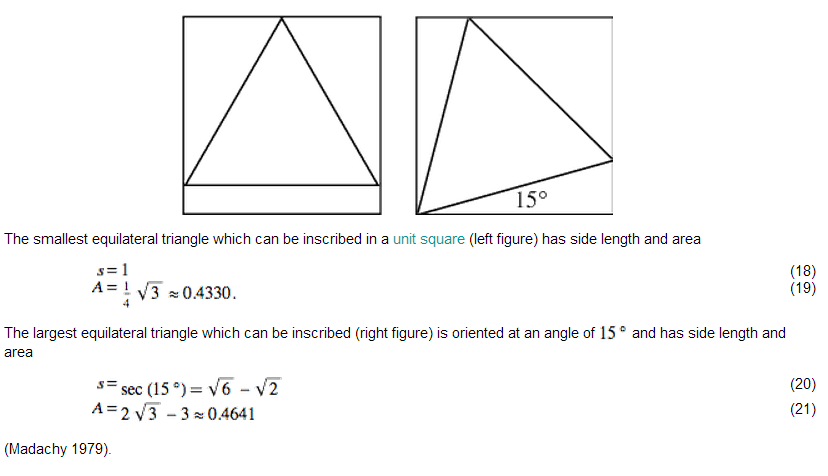
\includegraphics[scale=0.8]{hw8.png}
	\end{proof}
	
	\phantomsection
	\subsection*{{\color{purple}\underline{Problem 18}}}
	\addcontentsline{toc}{subsection}{\numberline{}Problem 18}
	Suppose that $f$ and $g$ are two differentiable functions which satisfy
	$fg' - f'g = 0$. Prove that if $f(a) = 0$ and $g(a) \neq 0$, then $f(x) = 0$
	for all $x$ in an interval around $a$.
\begin{proof}
	On any interval where $h(x) = \dfrac{f(x)}{g(x)}$ is defined, it is differentiable
	and by hypothesis,
	$$h'(x) = \dfrac{g(x)f'(x) - f(x)g'(x)}{g(x)^2} = 0$$ so $f/g$ is constant on 
	that interval. So if $f(a) = 0$, then $f(x) = 0$ in an interval around $a$
	which $g \neq 0$.
\end{proof}
	
	\phantomsection
	\subsection*{{\color{purple}\underline{Problem 19}}}
	\addcontentsline{toc}{subsection}{\numberline{}Problem 19}
	\begin{enumerate}[(a)]
	\item Give an example of a function $f$ for which $\displaystyle\lim_{x\to \infty} f(x)$
	exists, but $\displaystyle\lim_{x\to \infty}f'(x)$ does not exist.
\begin{proof}
	An example is $f(x) = \dfrac{\sin(x^2)}{x}$, then $\displaystyle\lim_{x\to \infty}f(x) = 0$, but
	$$f'(x) = \dfrac{2x^2 \sin(x^2) - \sin(x^2)}{x^2}
	= 2\sin(x^2) - \dfrac{\sin(x^2)}{x^2}$$
	so $\displaystyle\lim_{x\to \infty}f'(x)$ does not exist.
\end{proof}	
	
	\item Prove that if $\displaystyle\lim_{x\to \infty}f(x)$ and 
	$\displaystyle\lim_{x\to \infty}f'(x)$ both exist, then $\displaystyle\lim_{x\to \infty}f'(x) = 0$.
\begin{proof}
	Let $L = \displaystyle\lim_{x\to \infty}f'(x)$. If $L < 0$ then there would be some $N$ 
	such that $|f'(x) - L| < \dfrac{|L|}{2}$ for $x > N$. This would imply that $f'(x) > \dfrac{|L|}{2}$.
	But that would imply, by the Mean Value Theorem that
	$$f(x) > f(N) + \dfrac{(x - N)|L|}{2} , \, \, \, \, \text{ for } x > N$$
	which would mean that $\displaystyle\lim_{x\to \infty}f(x)$ does not exists. Similarly,
	$\displaystyle\lim_{x\to \infty}f'(x)$ cannot be $< 0$.
\end{proof}
	
	\item Prove that if $\displaystyle\lim_{x\to \infty}f(x)$ exists and 
	$\displaystyle\lim_{x\to \infty}f''(x)$ exists, then $\displaystyle\lim_{x\to \infty}f''(x) = 0$.
	\begin{proof}
		Let $I = \displaystyle\lim_{x\to \infty}f''(x)$. If $L > 0$ then as in part (a),
		we have $\displaystyle\lim_{x\to \infty}f'(x) = \infty$. Apply the Mean Value
		Theorem shows that $\displaystyle\lim_{x\to \infty} f(x) = \infty$ contradicting
		the hypothesis. Similarly, $\displaystyle\lim_{x\to \infty}f''(x)$ cannot be $< 0$.
	\end{proof}
	\end{enumerate}
	
	\phantomsection
	\subsection*{{\color{purple}\underline{Problem 20}}}
	\addcontentsline{toc}{subsection}{\numberline{}Problem 20}
	Suppose that $f'(x) \geq M > 0$ for all $x \in [0, 1]$. Show that there is an interval
	of length $\dfrac{1}{4}$ on which $|f| \geq \dfrac{M}{4}$.
	\begin{proof}
	Note that $f$ is increasing. If $f(1/2) \geq 0$, then $f(3/4) \geq M/4$, so certainly
	$f \geq M/4$ on the interval $[3/4, 1]$. On the other hand, if $f(1/2) \leq 0$ then 
	$f(1/4) \leq -M/4$ so $f \leq -M/4$ on the interval $[0, 1/4]$.		
	\end{proof}
	
	
	\phantomsection
	\subsection*{{\color{purple}\underline{Problem 21}}}
	\addcontentsline{toc}{subsection}{\numberline{}Problem 21}	
	\begin{enumerate}[(a)]
	\item Suppose that $f'(x) > g'(x)$ for all $x$ and that $f(a) = g(a)$. Show that
	$f(x) > g(x)$ for $x > a$ and $f(x) < g(x)$ for $x < a$.
	\begin{proof}
	Apply the Mean Value Theorem to $f - g$. If $x > a$, then 
$$\dfrac{f(x) - g(x)}{x - a} = \dfrac{f(x) - g(x) -[f(a) - g(a)]}{x - a}
= f'(y) - g'(y) > 0 \text{ for some } y \in (a, x)$$
	Since $x - a > 0$, it follows that $f(x) - g(x) > 0$. Similarly, if $x - a < 0$,
	then $f(x) < g(x)$.	
	\end{proof}
	
	\item Show an example that these conclusion do not follow without the hypothesis
	$f(a) = g(a)$. \\
	\includegraphics[scale=1.0]{hw81.png} \\
	\item Suppose that $f(a) = g(a)$, and that $f'(x) \geq g'(x)$ for all $x$, and that
	$f'(x_0) > g'(x_0)$ for some $x_0 > a$. Show that $f(x) > g(x)$ for all $x \geq x_0$.
	\begin{proof}
		An argument similar to that for part (a) shows that $f(x) \geq g(x)$ for all 
		$x > a$. More generally, $(f - g)(y) \geq (f - g)(x)$ for $a < x < y$. If we
		had $0 = f(x_0) - g(x_0) = (f - g)(x_0)$, then since $(f - g)(a) = 0$, we could
		have $(f - g)$ constant on $[a, x]$. But then we could not have $(f - g)'(x_0) > 0$.
		So we have $(f - g)(x_0) > 0$ which then implies that $(f - g)(x) > 0$ for all $x > x_0$.		
	\end{proof}
	\end{enumerate}		
	
		
	\phantomsection
	\subsection*{{\color{purple}\underline{Problem 22}}}
	\addcontentsline{toc}{subsection}{\numberline{}Problem 22}	
	Let $a \neq 0$ and $n$ be even. Prove that the polynomial
	equation $x^n + a^n = (x + a)^n$ has exactly one (real) solution.
	\begin{proof}
	Note first that if $n$ is even, then $n − 1 > 1$ is
	odd and the function $g(x) = nx^{n-1}$ is strictly increasing (in
		particular, one-one).
	Let $f(x) = (x + a)^n - x^n - a^n$. If $f(x_0) = 0$ for some
	$x_0 \neq 0$, then $f'(c) = 0$ for some $c$ between $0$ and $x_0$, 
	by Rolle’s Theorem. But $f'(x) = n(x + a)^{n-1} - nx^{n-1}$, so that
	$f'(c) = 0$ implies that $g(c + a) = g(c)$, contradicting that $g$ is
	one-one.
	\end{proof}
	
	\phantomsection
	\subsection*{{\color{purple}\underline{Problem 23}}}
	\addcontentsline{toc}{subsection}{\numberline{}Problem 23}
	\begin{enumerate}[(a)]
		\item Give an example of a continuous function on $(0, 1)$ which is bounded
		but attains neither a maximum nor a minimum value.
		\begin{proof}
			The function $f(x) = x$ for $x \in (0, 1)$ has $\sup\{f(x) : 0 < x < 1\} = 1$
			and $\inf\{f(x) : 0 < x < 1 \} = 0$, but $0 < f(x) < 1$ for all $x \in (0, 1)$.
		\end{proof}
		
		\item Suppose that $f$ is continuous on $\mathbb{R}$ and that for any number
		$M$ there exists $\delta > 0$ such that $f(x) > M$ if $|x| > \delta$. Prove 
		that $f$ attains a min.
		\begin{proof}
			Let $M = f(0)$ and let $\delta$ be such that $f(x) > f(0)$ for $|x| > \delta$.
			The function $f$ is continuous on the compact interval $[\delta, \delta]$, 
			so $f$ attains a min value in that interval; that is there is $y \in [-\delta, \delta]$
			such that $f(x) \geq f(y)$ for all $x \in [-\delta, \delta]$. In particular
			$f(0) \geq f(y)$ and thus $f(x) \geq f(0) \geq f(y)$ for all $x$ such that
			$|x| > \delta$.
		\end{proof}
	\end{enumerate}
	
	\phantomsection
	\subsection*{{\color{purple}\underline{Problem 24}}}
	\addcontentsline{toc}{subsection}{\numberline{}Problem 24}
	Prove that $f(x) = \sqrt{x}$ is uniformly continuous on $(1, \infty)$. 
	\begin{proof}
		If $x, y > 1$, then $\dfrac{1}{\sqrt{x} + \sqrt{y}} < \dfrac{1}{1 + 1} = \dfrac{1}{2}$.
		Rationalizing yields,
		\begin{eqnarray*}
			|\sqrt{x} - \sqrt{y}| &=& \dfrac{|\sqrt{x} - \sqrt{y}|(\sqrt{x} + \sqrt{y})}{\sqrt{x} + \sqrt{y}} \\
			&=& \dfrac{|x - y|}{\sqrt{x} + \sqrt{y}} < \dfrac{1}{2}|x - y|
		\end{eqnarray*}
		Therefore given $\epsilon > 0$, take $\delta = 2\epsilon$, then if $|x - y| < \delta$, then
		$|\sqrt{x} - \sqrt{y}| < \dfrac{1}{2} \cdot 2 \epsilon = \epsilon$.
	\end{proof}
	
	\phantomsection
	\subsection*{{\color{purple}\underline{Problem 25}}}
	\addcontentsline{toc}{subsection}{\numberline{}Problem 25}
	Suppose that $f$ were continuous on $[a, b]$ but not bounded on $[a, b]$, then $f$ would
	be unbounded on either $[a, (a+b)/2]$ or $[(a + b)/2, b]$. 
	\begin{proof}
	Let $c$ be in each $I_n$. Since $f$ is continuous at $c$, there is $\delta > 0$ such that
	$f$ is bounded on the set of all points in $[0, 1]$ satisfying $|x - c| < \delta$. 
	Choose $n$ with $\dfrac{1}{2^n} < \delta$. Since $c$ is in $I_n$, all points
	$x$ of $I_n$ satisfy $|x - c| < \delta$. This contradicts the fact that $f$
	is not bounded on $I_n$.
	\end{proof}
	
	\phantomsection
	\subsection*{{\color{purple}\underline{Problem 26}}}
	\addcontentsline{toc}{subsection}{\numberline{}Problem 26}
	Determine (either prove or give a counterexample) whether the following statements are true: (a) The union of two
uncountable sets is uncountable. (b) The intersection of two uncountable sets is uncountable.
	\begin{proof}
	(a) True. If $A \cup B$ is countable, then there is a one-one mapping $f : A \cup B \rightarrow N$. 
	The composite $f \circ i : A \rightarrow
A \cup B \rightarrow N$ is one-one, and hence A is countable. 
(b) False. $A = (−\infty, 1]$ and $B = [1, \infty)$ are uncountable but $A \cap B = \{1\}$ is countable.
	\end{proof}
	
	\phantomsection
	\subsection*{{\color{purple}\underline{Problem 27}}}
	\addcontentsline{toc}{subsection}{\numberline{}Problem 27}
	Prove that $a_n = \dfrac{2n - 1}{n + 3}$ converges to $L = 2$.
	\begin{proof}
	Given $\epsilon > 0$, let $N = \max(2, 7/\epsilon - 2)$. If $n > N$, then
	$$\bigg|\dfrac{2n - 1}{n + 3} - 2\bigg| = \dfrac{7}{N + 3} < \epsilon$$
	\end{proof}		
	
	
	\phantomsection
	\subsection*{{\color{purple}\underline{Problem 28}}}
	\addcontentsline{toc}{subsection}{\numberline{}Problem 28}
	Suppose that $a$ and $b$ are two consecutive roots of the polynomial function $f$, but that
	$a, b$ are not double roots, we can write $f(x) = (x - a)(x - b)g(x)$ where $g(a) \neq 0, g(b) \neq 0$.
	\begin{enumerate}[(a)]
		\item Prove that $g(a), g(b)$ have the same sign.
		\begin{proof}
		If $g(a)$ and $g(b)$ have opposite sign, then by Intermediate Value Theorem, there is $c \in (a, b)$
		such that $g(c) = 0 \Rightarrow f(c) = 0$, contradicting $a, b$ are consecutive roots of $f$.	
		\end{proof}				
		\item Prove that there is some number $x$ with $a < x < b$ and $f'(x) = 0$.
		\begin{proof}
			Because $a$ and $b$ are roots of $f$, $f(a) = f(b) = 0$. Moreover, $f$ is continuous on $[a, b]$
			and differentiable on $(a, b)$ because it is a polynomial. Thus by Rolle's Theorem, we have 
			that $f'(x) = 0$ for some $x \in (a,b)$. Note that the derivative $f'(x) = (x - a)g(x) +
			(x - b)g(x) + (x - a)(x - b)g'(x)$, so that $f'(a) = (a - b)g(a) \neq 0$ and $f'(b) = (b - a)g(b) \neq 0$.
		\end{proof}
	\end{enumerate}
	
	\phantomsection
	\subsection*{{\color{purple}\underline{Problem 29}}}
	\addcontentsline{toc}{subsection}{\numberline{}Problem 29}
	Let $f(x) = |x|^3$. Find $f'(x), f''(x)$, and find all numbers $x$ for which $f'''(x)$ exists. 
	\begin{proof}
		We have
		$$
		f(x) = 
		\begin{cases}
			x^3 &, \text{ if } x \geq 0 \\
			-x^3 &, \text{ if } x < 0		
		\end{cases}
		$$
		Hence
		$$
		f'(x) = 
		\begin{cases}
			3x^2 &, \text{ if } x \geq 0 \\
			-3x^2 &, \text{ if } x < 0		
		\end{cases}
		$$
		For $x = 0$, we find
		$$\displaystyle\lim_{h\to 0}\dfrac{f(0 + h) - f(0}{h} = \displaystyle\lim_{h\to 0}\dfrac{|h|^3}{h} = 
		\displaystyle\lim_{h\to 0} h \cdot |h| = 0$$
		and we obtain that $f'(x) = 3x|x|$.
		Similarly, we have
		$$
		f''(x) = 
		\begin{cases}
			6x &, \text{ if } x \geq 0 \\
			-6x &, \text{ if } x < 0		
		\end{cases}
		$$
		For $x = 0$, we have
		$$f''(0) = \displaystyle\lim_{h\to 0} \dfrac{f'(h) - f'(0)}{h} = \displaystyle\lim_{h\to 0} \dfrac{3h|h|}{h} = 0$$
		and we obtain $f''(x) = 6|x|$ for all $x$.
		It follows by similar arguments that $f'''(x) = 6 \dfrac{|x|}{x}$ if $x \neq 0$, and that $f'''(0)$ does not exist.
	\end{proof}
	
	
	
\end{document}
